%!TEX root = ../rapport.tex
%!TEX encoding = UTF-8 Unicode
\chapter{Simulation temps réel - Opal-RT}
Ce chapitre présente les principaux domaines d'utilisation d'un simulateur temps-réel comme ceux produits par la compagnie Opal-RT ainsi que la validation croisée entre SPS et le simulateur temps réel pour la simulation du hacheur 4 quadrants simple.

\section{Cas typiques d'utilisation d'un simulateur temps-réel}
Le simulateur temps-réel possède trois cas typiques d'utilisation. Premièrement, le simulateur temps-réel permet d'effectuer de la modélisation de type "Hardware-in-the-loop". Dans ce type d'essai, le simulateur temps-réel modélise un système comme un réseau électrique de grande envergure, un parc éolien ou l'alimentation d'un appareillage spécifique. À l'aide de cette modélisation et des différents modules d'entrées-sorties du simulateur, il est possible d'interagir avec plusieurs types de modules de contrôle. Ainsi, il n'est pas nécessaire de faire des essais directement sur le réseau ou sur les machines de grande envergure.

\paragraph{} Deuxièmement, le simulateur temps-réel peut effectuer le rôle de contrôleur. En effet, il suffit d'implanter le module de contrôle à l'intérieur du simulateur et de connecter celui-ci sur le réseau ou sur l'appareillage qui doit être contrôlé, afin d'effectuer les différents essais nécessaires permettant d'optimiser les paramètres de contrôle.
\paragraph{} Finalement, le troisième cas type est l'assemblage des deux types de simulations. En simulant le contrôle de l'équipement ainsi que l'équipement lui-même, il est possible de faire différents essais en peu de temps, sachant que le simulateur est capable d'effectuer la simulation en temps réel avec un pas de calcul très faible.

\section{Simulation du hacheur 4 quadrants sur Opal-RT}
Pour effectuer l'implantation du hacheur 4 quadrants sur Opal-RT, plusieurs étapes ont été nécessaires afin d'obtenir les résultats recherchés. En effet, la suite de logiciels fournie par Opal-RT manque beaucoup de convivialité et la documentation possède beaucoup de zones grises. Beaucoup d'essais par tâtonnement sont nécessaires pour implanter la simulation. De plus, comme le simulateur doit s'interfacer avec Matlab, celui-ci est dépendant des versions installées. Ainsi, lors de nos différents essais, il a fallu retrouver une version de Matlab 2011b pour que tous les outils d'Opal-RT soient fonctionnels. Une fois les différents logiciels nécessaires installés et fonctionnels, il a été possible d'implanter la simulation du hacheur 4 quadrants en utilisant les renseignements obtenus lors de notre formation sur le simulateur temps réel. Toutefois, effectuer la conversion d'une simulation SPS vers une simulation Opal-RT n'est pas réellement ardu. 

\paragraph{} Une fois venu le temps d'exploiter la simulation, plusieurs pépins ont été rencontrés au niveau de l'affichage des courbes en temps réel ainsi qu'au niveau de la précision des résultats. Il a été nécessaire de jouer avec les paramètres de communication entre Matlab et le simulateur pour obtenir le résultat recherché. Finalement, suite à plusieurs interactions avec l'assistance technique d'Opal-RT, il a été possible d'obtenir un résultat acceptable. Les figures \ref{DC_ch_H4Q_1} et \ref{DC_ch_H4Q_2} montre le courant obtenu dans l'électroaimant pour un pas de calcul de 25 $\mu$s. On remarque que le simulateur présente la dynamique recherchée. L'ondulation de courant possède une fréquence d'environ 1 kHz comme spécifié et le courant possède une ondulation crête à crête d'environ 20 A. Cette valeur est un peu différente de la simulation de SPS, car la fréquence de commutation réelle de SPS est un peu plus élevée ce qui permet une amplitude d'ondulation un peu plus petite. Toutefois, cette différence est minime et peut aussi provenir des différences au niveau de la discrétisation des interrupteurs entre Opal-RT et SPS. De plus, le pas de calcul étant largement supérieur à celui de SPS, il se peut que les valeurs en aient été affectées. 

 \begin{figure}[htb]
 \centering
 \makebox[\textwidth][c]{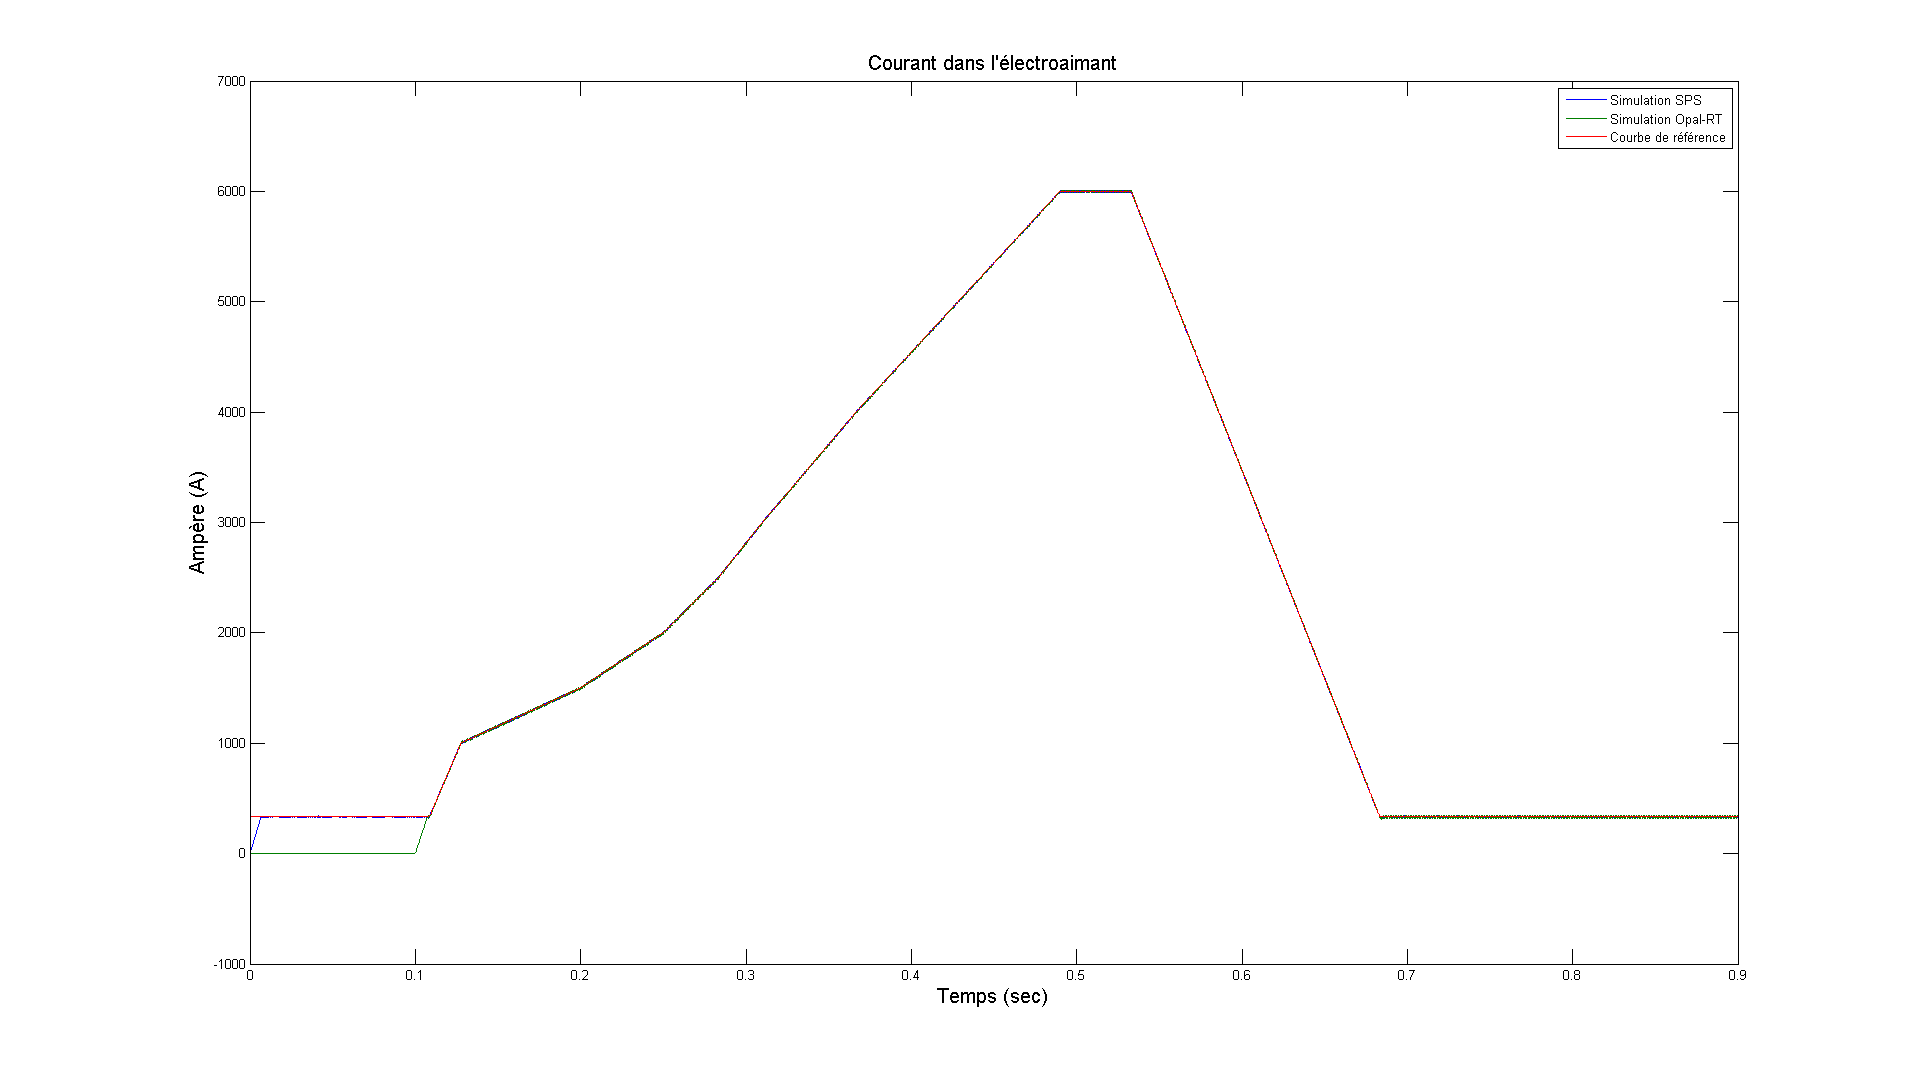
\includegraphics[width=0.95\textwidth]{fig/Opal-RT_Courant.png}}
 \caption{Courant traversant la charge sur Opal-RT et SPS pour un pas de calcul de 25$\mu$s pour le hacheur 4 quadrants (Affichage de 0.9 seconde)}
 \label{DC_ch_H4Q_1}
 \end{figure}

  \begin{figure}[htb]
 \centering
 \makebox[\textwidth][c]{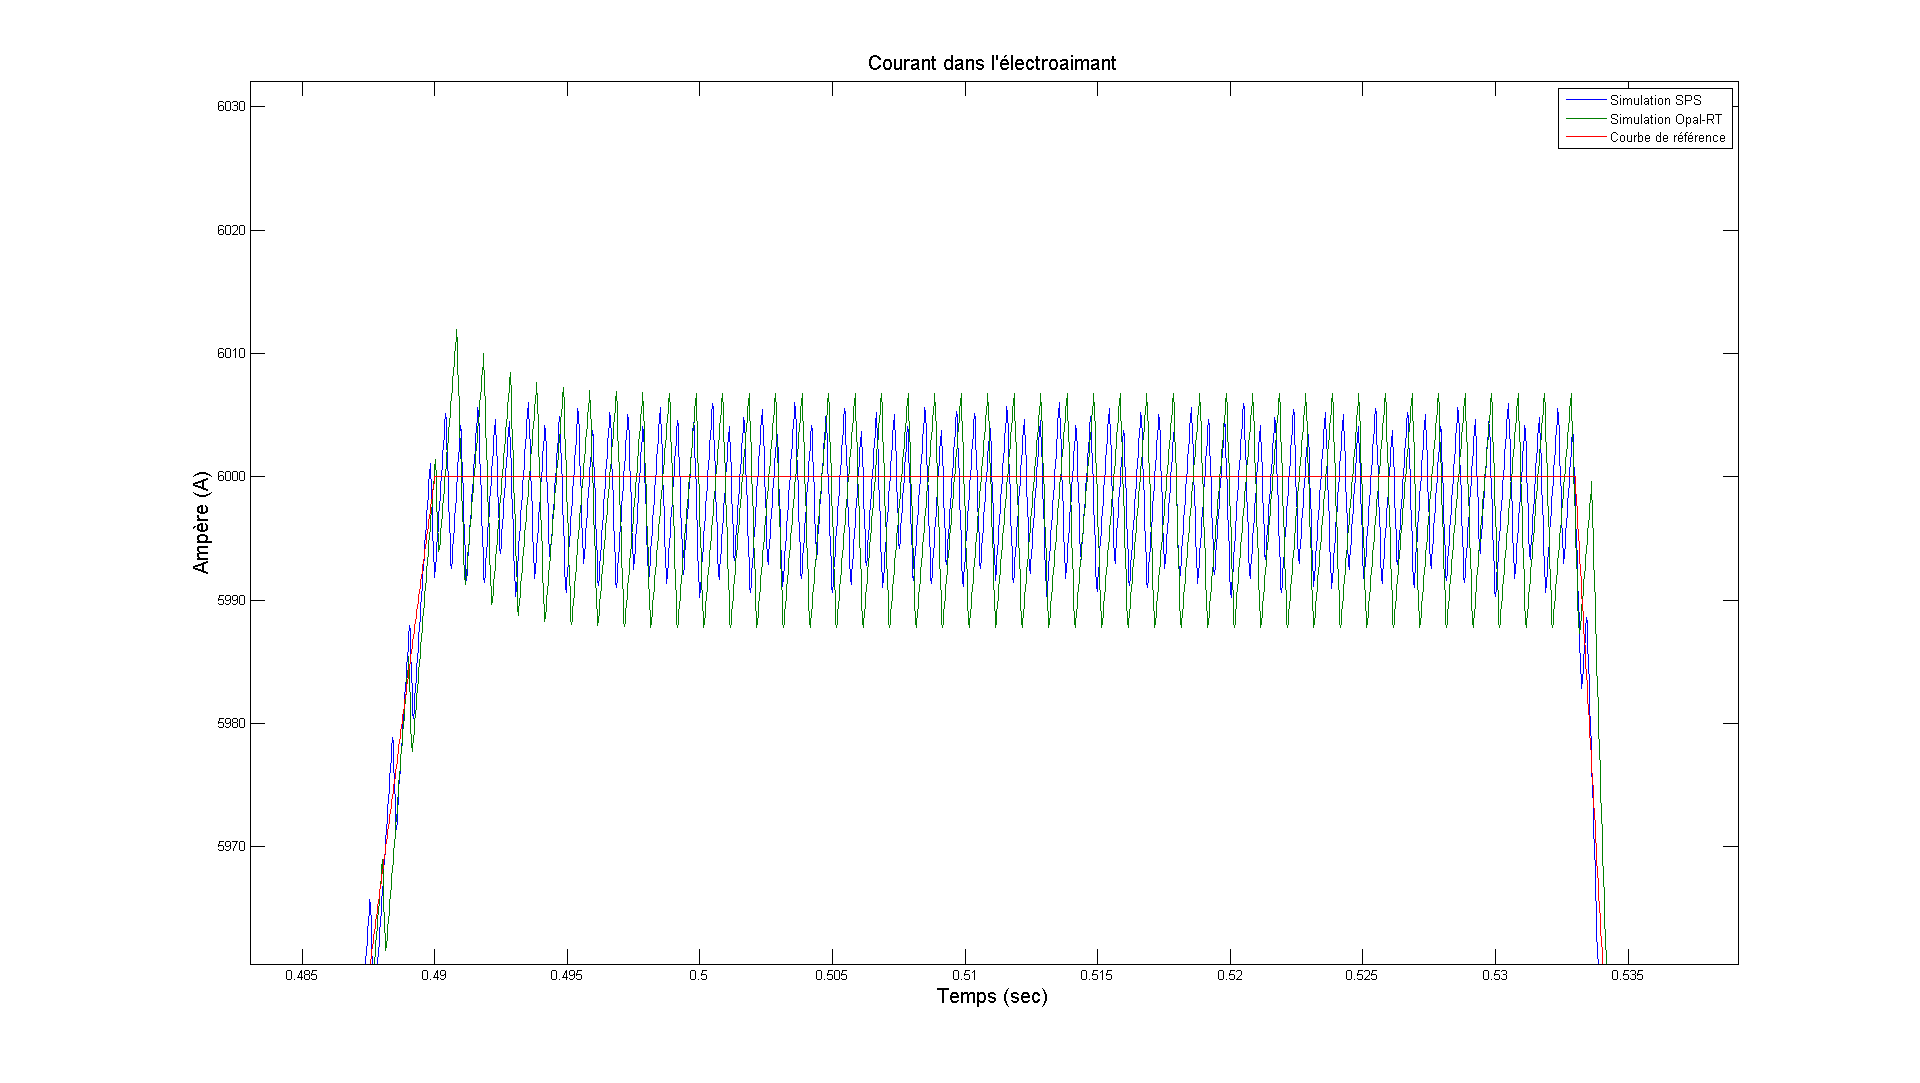
\includegraphics[width=0.95\textwidth]{fig/Opal-RT_Courant2.png}}
 \caption{Courant traversant la charge sur Opal-RT et SPS pour un pas de calcul de 25$\mu$s pour le hacheur 4 quadrants (Affichage de 5ms)}
 \label{DC_ch_H4Q_2}
 \end{figure}





